\begin{marginfigure}
\begin{tikzpicture}
\node [name-dest] (box){%
    \begin{minipage}{0.80\textwidth}
     \begin{itemize}
    \item Rhys Tyers
    \item Dave Kirkpatrik
    \item Christ Keeley
    \item Dave Wilson
    \item Pete Hambley
    \end{itemize}
    \end{minipage}

};
\node[fancytitle, right=10pt] at (box.north west) {Jailbreak};
\end{tikzpicture}
\end{marginfigure}

\section{Discovery of Jailbreak}
 
A group of us were meandering across the western edge of the plateau. Dewi and Dave had been poking in all the B series of the holes. I had my fair share of being inserted into exactly Rhys shaped holes, a couple of which went further than my body length.
 
It was sunny, we were happy to be in the open air. As we neared the cliff in an inconspicuous valley I spot a couple of small holes right next to each other. Peering in they immediately join up, the pillar in the center forming a single bar, barring our entrance (ha). Beyond a dusty body sized tube invited us in. 
We each had a go with the hammer. Trying to chip at the solid rock bar. Chris Keeley steps up and from somewhere deep within unleashes the power of Thor. Thousands of hours of metal music and the power of long forgotten Norse mythology flowing through his long golden hair. He screams and attacks the rock, again and again and again. Within a few minutes its gone, all that’s left are two sharpish protrusions and a lot of rock flour littering the grassy bank. 
 
As the most sinous caver present (that had his caving kit) I am given the honour of inserting myself first. It’s a helmet off affair. Slither, slither, cough, cough, fuck thats dusty. I pop out into a swiss cheese chamber. Lots of little holes leading off. Most die very quickly. Through one, 30cm in diameter, there is daylight and Dewi gets a photo of me in there. One is very interesting though. Drawing a small draft I follow it and it drops, 90 degrees downwards. Gosh, a pitch. Could it go?
 
We return later. Me, DKP and Chris Keeley. I place a bolt or two, so does DKP. DKP descends first. The pitch, beautifully white and clean, we call \emph{Isengard}. I ask how it looks. 

\begin{figure*}[t!]
\checkoddpage \ifoddpage \forcerectofloat \else \forceversofloat \fi
\centering
\begin{subfigure}[t]{0.42\textwidth}
\centering
\frame{\includegraphics[width=\linewidth]{"images/2013/rhys-jailbreak-2013/pete-hambley-jailbreak__1_".jpg}}
 \caption{}\label{water chamber below helm's deep}
\end{subfigure}
    \hfill
    \begin{subfigure}[t]{0.56\textwidth}
        \centering
        \frame{\includegraphics[width=\linewidth]{"images/2013/rhys-jailbreak-2013/pete_jailbreak__1_".jpg}} 
        \caption{} \label{HelmsDeep}
    \end{subfigure}
    
    \vspace{0.3cm}
    \begin{subfigure}[t]{\textwidth}
    \centering
        \frame{\includegraphics[width=\linewidth]{"images/2013/rhys-jailbreak-2013/rhys-jailbreak__1_".jpg}} 
        \caption{} \label{Touching the Void}
    \end{subfigure}
    \caption{
    \emph{a} After frantic bashing at the entrance squeeze Rhys attempts to break into the cave.
    \emph{b} Rhys inserting himself through the entrance squeeze
    \emph{c} At the bottom of Isengard pitch in the Barrows}
\end{figure*}





“Ummmmm............you should come down here”
 
Are there sweeter words to hear when caving? That unspoken divulgence that there is something indescribable or something better left to your own eyes to see. I bomb down the pitch and scramble up the bouldery passage at the bottom to join DKP. He is standing on the edge, where the passage intersects  a large chamber. Nice! Chris Keeley joins us and we excitedly bumble down into the chamber.
 
There are a series of chambers in fact, joined by low sections. To the South they head upwards and veer towards to the cliff face. The floor get closer to the ceiling. There are a couple of 2m deep holes in the floor, nearly the size of the chamber, leaving just a ledge around the edge to climb around on. At the end the floor reaches near the ceiling and further passage is choked with choss. Through a crack in the wall you can perhaps see a smidgen of daylight.
 
We climbed down into a couple of the holes, most have nothing of interest in. One has a narrow bedding plain that you can crawl further into. We would spend a little while on a subsequent trip trying to dig this without much success. 
 
Heading North from where we originally dropped in, a low pebbly crawl brings you into another large chamber. The floor is rocks and boulders and they dip towards the center, maybe a dig? At the far end a drip has carved a narrow tube downwards next to the wall. We have a poke at it. And its got a few rocks blocking the way. On a subsequent trip we set up a rather elaborate (read basic) hauling  system and move a huge rock out of there. Down 6m or so a floor is reached and an impossibly tight beeding plain heads off.
 
We name our find \emph{The Barrows} due to it’s dead nature. Who knows there might be more but it’s so close to the cliff that any small ways on seem to have been shattered and filled with choss.

\name{Rhys Tyers}

\begin{figure*}[t!]
\checkoddpage \ifoddpage \forcerectofloat \else \forceversofloat \fi
\centering
\frame{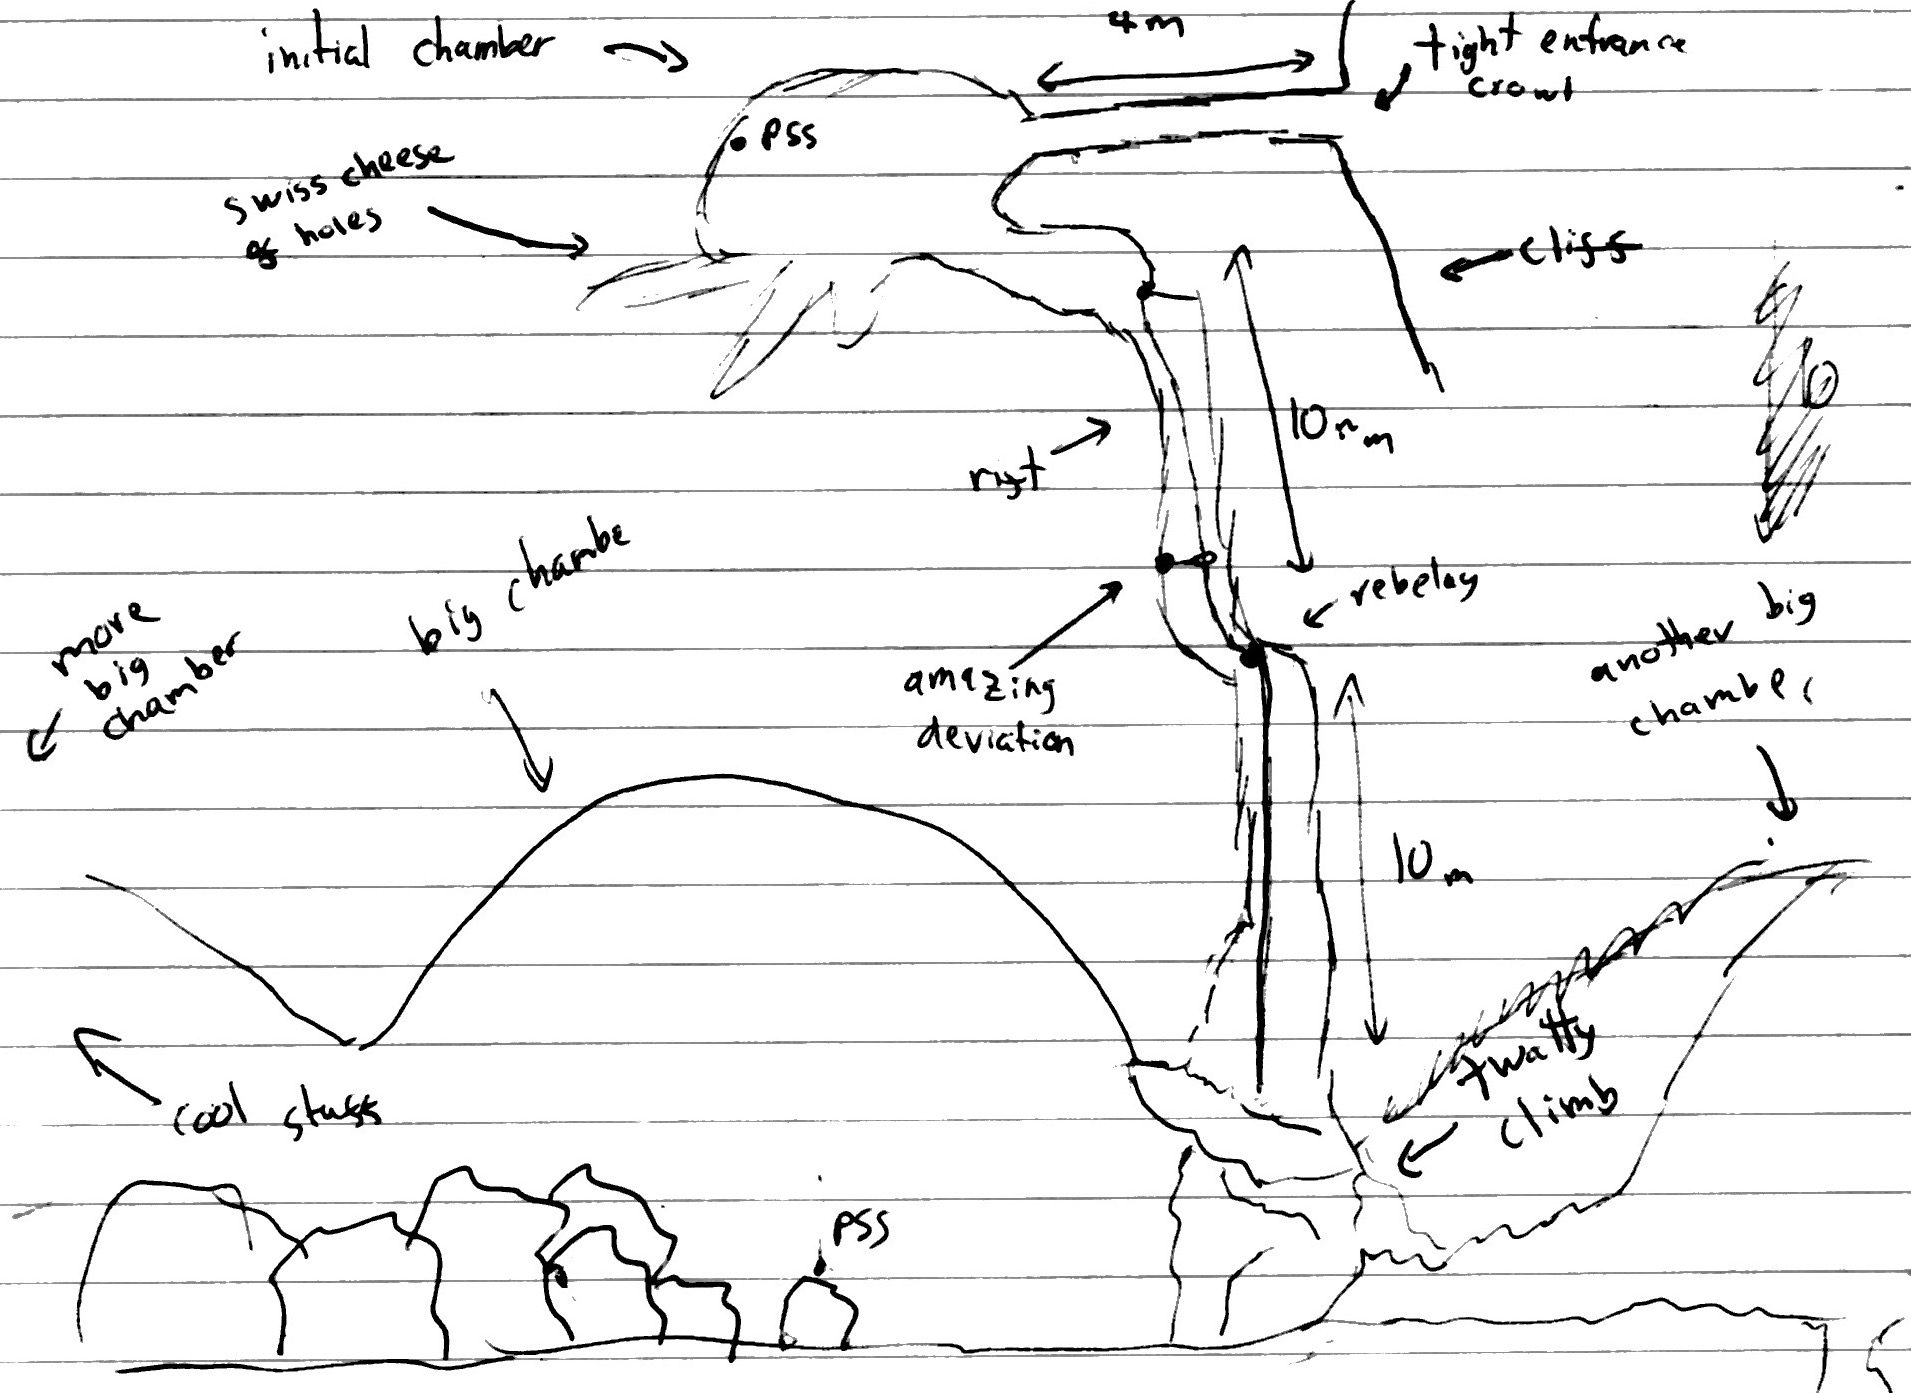
\includegraphics[width=\textwidth]{images/2013/rhys-jailbreak-2013/jailbreak.jpg}}
\caption{An extended elevation of Jailbreak cave, drawn in the 2013 scanned logbook --- scanned, from Rhys Tyers }
\label{ee jailbreak}
\end{figure*}



